% !TEX root=../../Thesis.tex
\chapter{Accounting for the uncertainty}\label{ch:uncertainty}
% \begin{center}
% 	\textit{\textbf{RQ 2: In what way can an \gls{rl} agent utilize the uncertainty of its predictions and actions?}}
% 	% \textit{\textbf{RQ 4: How can the quality of a RL agent be improved by accounting for uncertainty?}}
% 	\end{center}
% 	\vspace{12pt}

The previous chapter formulated the \gls{pomdp} and introduced how deep Q-learning methods can be utilized to create decision-making agents capable of navigating intersections. A significant advantage of RL methods is their scalability to different scenarios through appropriate training. However, a drawback of deep Q-learning methods, is the use of neural networks, which provide a black-box solution without indicating any confidence or uncertainty in their decisions.

This chapter presents two approaches to estimating the uncertainty: \paperEnsamble addresses the uncertainty in the output of the \gls{dqn}, and \paperBelief addresses the uncertainty in the intention estimation that is fed as an input to the \gls{dqn}.

\section{Estimating the uncertainty of the Q-value}

To estimate the uncertainty of $Q$-estimate from the \gls{dqn}, \paperEnsamble employed statistical bootstrapping to train an ensemble of neural networks on different subsets of the available experience. This ensemble provides a distribution over the estimated $Q$-values. A better Bayesian posterior is obtained by adding different \gls{rpf} to each ensemble member~\cite{Osband2018}.
The $Q$-values of each ensemble member $k$ is then calculated as the sum of two neural networks, $f$ and $p$, with the same architecture, i.e.,
%
\begin{align}
	Q_k(s,a) = f(s,a;\theta_k) + \beta p(s,a;\hat{\theta}_k).
\end{align}
Here, the weights $\theta_k$ of network $f$ are trainable, and the weights $\hat{\theta}_k$ of the prior network $p$ are fixed to the randomly initialized values. A parameter $\beta$ scales the importance of the networks. With the two networks, the loss function in Eq.~\ref{eq:lossDQN} becomes
%
\begin{align}
	\label{eq:loss_boot}
	L(\theta_k) = \mathbb{E}_M \Big[ & (r + \gamma \max_{a'} (f_{\theta^-_k}+\beta p_{\hat{\theta}_k})(s',a') \nonumber \\
	& - (f_{\theta_k}+ \beta p_{\hat{\theta}_k})(s,a) )^2 \Big].
\end{align} 

% One limitation of the \gls{dqn} algorithm is that only the maximum likelihood estimate of the $Q$-values is returned. The risk of taking a particular action can be approximated as the variance in the estimated $Q$-value~\cite{Garcia2015}. 
% The basic idea is to train an ensemble of neural network on different subsets of the available experience. The ensemble will then provide a distribution of $Q$-values, which can be used to estimate the variance. Osband et al. extended the ensemble method by adding a \gls{rpf} to each ensemble member, which gives a better Bayesian posterior~\cite{Osband2018}. The $Q$-values of each ensemble member $k$ is then calculated as the sum of two neural networks, $f$ and $p$, with equal architecture, i.e.,
%

The training process of an ensamble \gls{rpf} is described by Algorithm~\ref{alg:ensamble_training}. 
An ensemble of $K$ \gls{dqn} are first initialized randomly. Each ensemble member is also assigned a separate experience replay memory buffer $m_k$. 
For each new episode, a random ensemble member $\nu$ is selected and used to take greedy actions throughout the episode, which corresponds to an approximate Thompson sampling approach to the exploration vs.~exploration dilemma.
Each new experience $e = (s_i, a_i, r_i, s_{i+1})$ is then added to the separate replay buffers $m_k$ with probability $p_\mathrm{add}$. The trainable weights of each ensemble member are then updated by uniformly sample a mini-batch $M$ of experiences and using \gls{sgd}.

\begin{algorithm}[h]
	\caption{Ensemble RPF training process}\label{alg:ensamble_training}
	\begin{algorithmic}[1]
		\For{$k \gets 1$ to $K$}
			\State Initialize $\theta_k$ and $\hat{\theta}_k$ randomly
			\State $m_k \gets \{\}$
		\EndFor
		\State $i \gets 0$
		\While{networks not converged}
			\State $s_i \gets $ initial random state
			\State $\nu \sim \mathcal{U}\{1,K\}$%, where $k \in \mathbb{N}$
			\While{episode not finished}
				\State $a_i \gets \argmax_{a} Q_\nu(s_i,a)$
				\State $s_{i+1}, r_i \gets $ \Call{StepEnvironment}{$s_i, a_i$}
				% \For{$i \in \{1,\dotsc,K\}$}
				\For{$k \gets 1$ to $K$}
					\If{$p \sim \mathcal{U}(0,1) < p_\mathrm{add}$}%, where $p \in \mathbb{R}$ 
						\State $m_k \gets m_k \cup \{(s_i, a_i, r_i, s_{i+1})\}$
					\EndIf
					\State $M \gets $ sample mini-batch from $m_k$
					\State update $\theta_k$ with SGD and loss $L(\theta_k)$
				\EndFor
				\State $i \gets i + 1$
			\EndWhile
		\EndWhile
	\end{algorithmic}
\end{algorithm}

The agent's uncertainty in choosing different actions can be defined as the coefficient of variation $c_\mathrm{v}(s,a)$ of the $Q$-values of the ensemble members. $c_\mathrm{v}(s,a)$ is then used to create a hard threshold $c_\mathrm{safe}$, which determines if an action has an acceptable level of uncertainty. 
A high uncertainty, where $c_\mathrm{v}(s,a) > c_\mathrm{v}^\mathrm{safe}$, indicates that $(s,a)$ is outside the training distribution. 
When the agent is fully trained, the policy $\pi$ chooses actions by maximizing the mean of the $Q$-values of the ensemble members, with the restriction $c_\mathrm{v}(s,a) < c_\mathrm{v}^\mathrm{safe}$, i.e.,
%
\begin{equation}
	\begin{aligned}
		\pi = \argmax_{a} \frac{1}{K} \sum_{k=1}^K Q_k(s,a),\\
		\textrm{s.t.} \quad c_\mathrm{v}(s,a) < c_\mathrm{v}^\mathrm{safe}.
	\end{aligned}
\end{equation}
%
% In a situation where no possible action fulfills the confidence criterion, a fallback action $a_\mathrm{safe}$ is chosen.

%  In this thesis, the benefit of this estimate is demonstrated by applying a backup policy $\pi_\mathrm{backup}(s)$ if an action has an unacceptable level of uncertainty, i.e., the trained agent follows the policy
% %
% \begin{align}
%     \pi_{\sigma_\mathrm{e}}(s) = 
%     &\begin{cases} \argmax_{a} \mathbb{E}_k[Q_k(s,a)], & \mathrm{if\ } \mathrm{Var}_k[Q_k(s,a)] < \sigma^2_\mathrm{e}, \\
%     \pi_\mathrm{backup}(s), & \mathrm{otherwise}.
%     \end{cases}
% \end{align}






\section{Estimating the uncertainty of the input}

As previously mentioned in Section~\ref{sec:pomdp_statespace}, the state space of the intersection problem considered in this thesis consists of position, velocity and the intention of the surrounding driver. While the position and velocity are observable states, the intention state is not directly observable. The hypothesis in \paperLSTM was that the hidden state in the \gls{lstm} layer would incorporate some estimation of intentions. 

Upon analyzing the scenarios that led to collisions, it was observed that the agent often quickly entered a state where a collision could occur if both parties maintained the same velocity. However, due to the black-box nature of the system, it is impossible to determine when this state incorrectly estimated the intention. The policy generally positioned the agent in a way that avoided conflicts with other cars' time to intersection, preventing many collisions. Nonetheless, in cases where the cars did collide, the agent somehow ended up on a collision course and struggled to navigate out of it.

% Because the state is no longer observable, the agent must reason about the history of taken actions and observations. Often, this history can be summarized in a statistic refered to as a belief, or belief state. A belief is a probability distribution over states so that $b: \mathcal{S} \rightarrow [0,1]$ and $\sum_{s} b(s)=1$, or $\int_{s} b(s)=1$ for continuous states. 

In \paperBelief,  two methods are proposed for representing belief over drivers' intentions using a particle-based approach and a compact parametric representation, which can manifest as a probability distribution (QID) or a point estimate (QMDP-IE).

Our proposed particle filter exhibited promising results in estimating intention probabilities.
% , although improvements potentially could be made through enhanced prediction models and increased computational resources. 
We leveraged these intention probability estimates in QMDP-IE and QID algorithms, which demonstrated superior performance compared to respective baseline approaches QMDP and QPF. QMDP-IE, in particular, offered adjustable aggressiveness post-training, yielding a collision rate close to the Oracle DQN with an optimal threshold value $\zeta_\mathrm{threshold}$.
Furthermore, QID policies collision rate was comparable to QMDP-IE for conflict scenarios. 



\section{Using the uncertainty estimate}

With an estimate of the uncertainty in actions we showed that it can be used to reduce collisions and risk by choosing another policy than the one trained on data it is not confident in. 

\begin{figure}[h]
	\mbox{\parbox{\textwidth}{
	\centering
	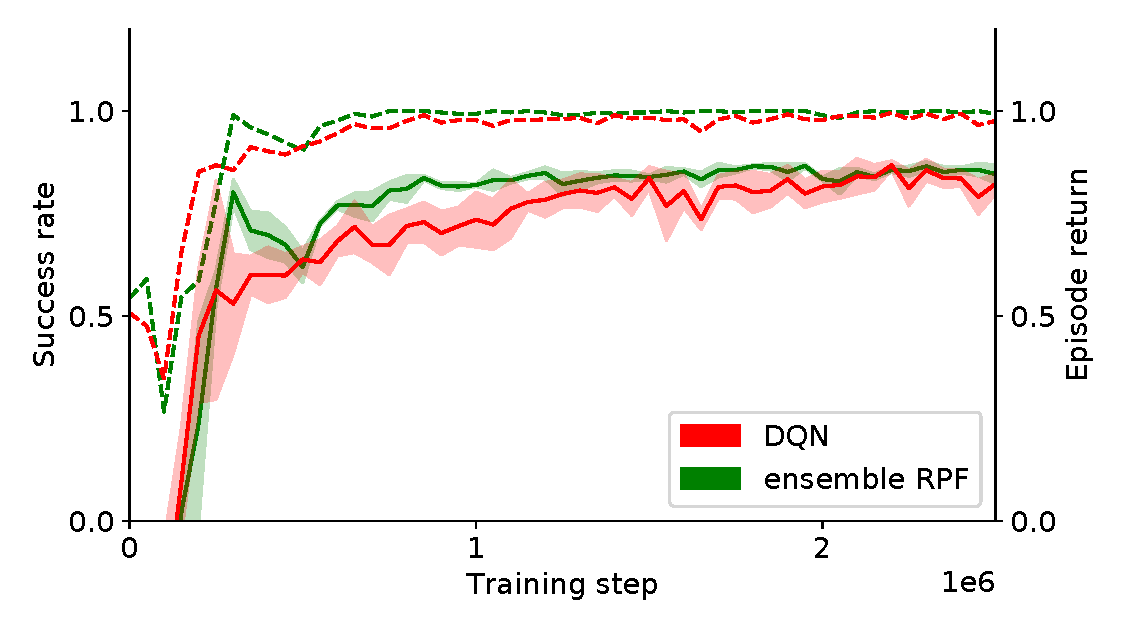
\includegraphics[width=0.7\columnwidth]{YourThesis/papers/ensamble/figures/return_success_rate_2_wo_type_3_fonts.pdf}
	}}
	\caption{Proportion of test episodes where the ego vehicle reached its goal (dashed), and episode return (solid), over training steps for the ensemble RPF and DQN methods. The shaded areas show the standard deviation for $5$ random seeds.}
	% \label{fig:returnAndSuccess}
\end{figure}

% \begin{figure}[h]
% 	\mbox{\parbox{\textwidth}{
% 	\centering
% 		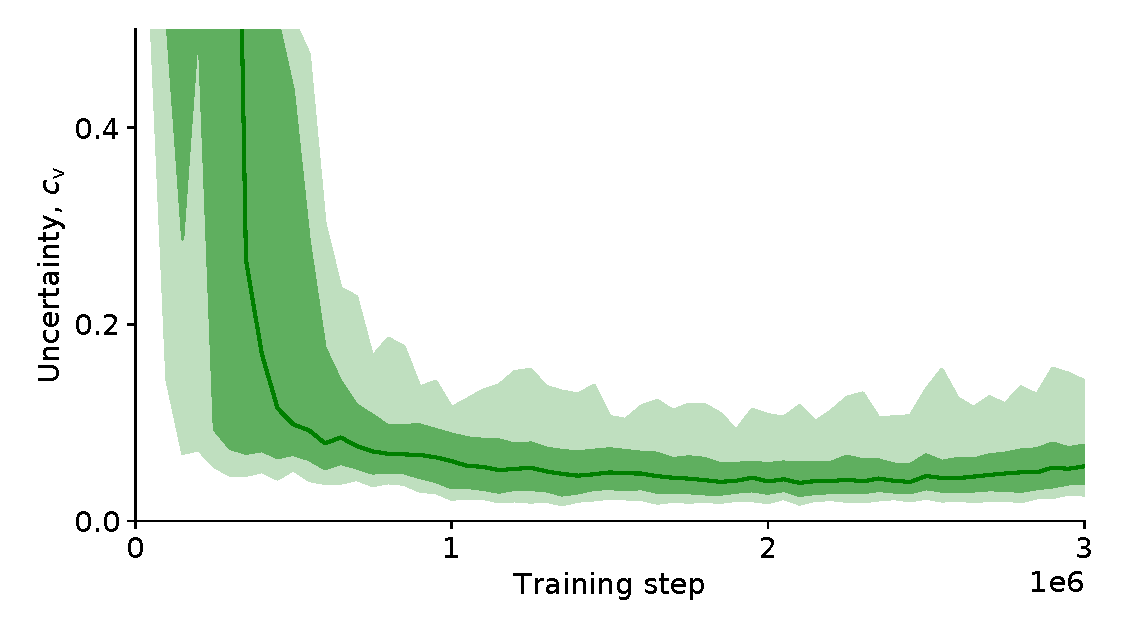
\includegraphics[width=0.7\columnwidth]{YourThesis/papers/ensamble/figures/uncertainty_3_wo_type_3_fonts.pdf}
% 		}}
% 		\caption{Mean coefficient of variation $c_\mathrm{v}$ for the chosen action during the test episodes. The dark shaded area shows percentiles $10$ to $90$, and the bright shaded area shows percentiles $1$ to $99$.}
% 	% \label{fig:cv}
% \end{figure}

\begin{figure}[h]
	\mbox{\parbox{\textwidth}{
	\centering
		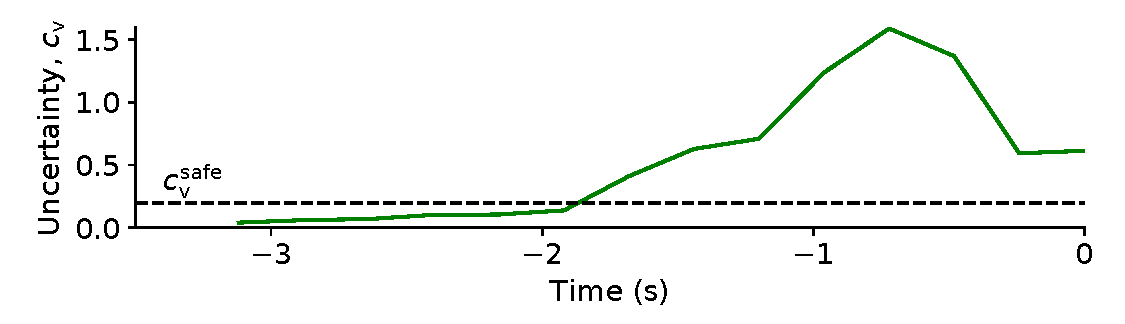
\includegraphics[width=0.8\columnwidth]{YourThesis/papers/ensamble/figures/uncertainty_at_collision_wo_type_3_fonts.pdf}
		}}
		\caption{Uncertainty $c_\mathrm{v}$ during the time steps before one of the collisions in the test episodes, within the training distribution. The collision occurs at $t=0$ s.}
	% \label{fig:cvDuringCrash}
\end{figure}

\begin{figure}[h]
	\mbox{\parbox{\textwidth}{
		\centering
	\begin{subfigure}[]{0.9\columnwidth}
	\centering
		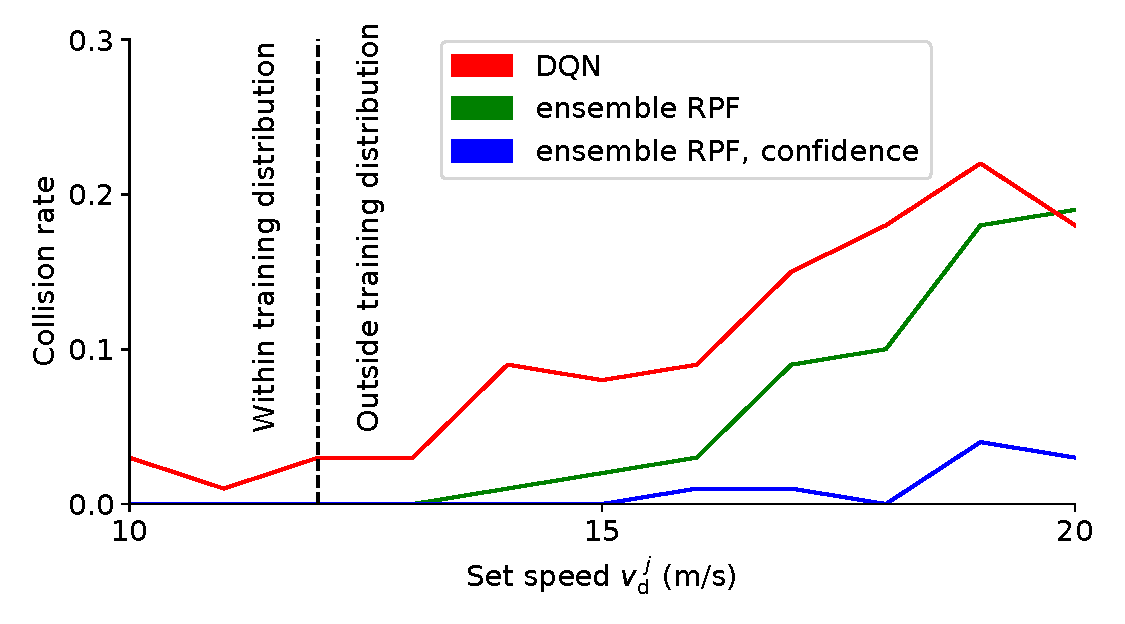
\includegraphics[width=0.7\columnwidth]{YourThesis/papers/ensamble/figures/collisions_outside_distribution_2_wo_type_3_fonts.pdf}
		\caption{Proportion of collisions.}
	\end{subfigure}
	
	\vspace{5pt}
	
	\begin{subfigure}[]{0.9\columnwidth}
	\centering
		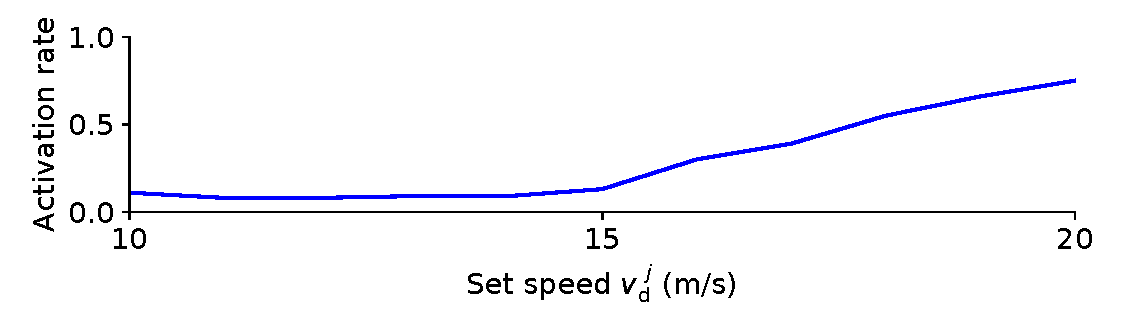
\includegraphics[width=0.7\columnwidth]{YourThesis/papers/ensamble/figures/activation_rate_2_wo_type_3_fonts.pdf}
		\caption{Proportion of episodes where $a_\mathrm{safe}$ was used at least once.}
	\end{subfigure}
	\caption{Performance of the ensemble RPF agent, with and without the confidence criterion, and the DQN agent, in test episodes with different set speeds $v_\mathrm{d}^j$ for the surrounding vehicles. %The shaded areas show the standard deviation for $5$ random seeds.
	}
	}}
	% \label{fig:performanceOutsideDistribution}
\end{figure}

% \begin{figure}[h]
% 	\mbox{\parbox{\textwidth}{
% 	\centering
% 	\begin{subfigure}[t]{0.48\columnwidth}
% 		\centering
% 		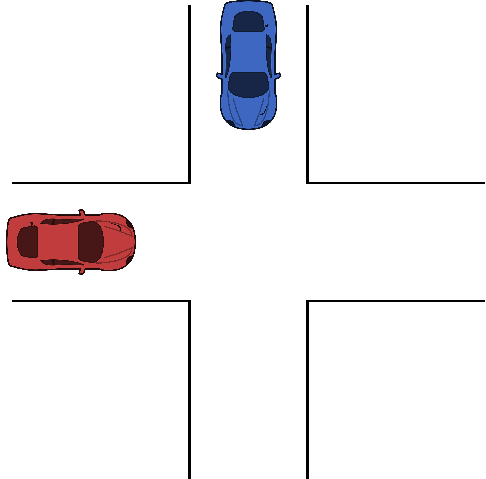
\includegraphics[width=0.7\columnwidth]{YourThesis/papers/ensamble/figures/figures-scen1.pdf}
% 		\caption{$t=0$, initial situation.}
% 	\end{subfigure}%
% 	~ 
% 	\begin{subfigure}[t]{0.48\columnwidth}
% 		\centering
% 		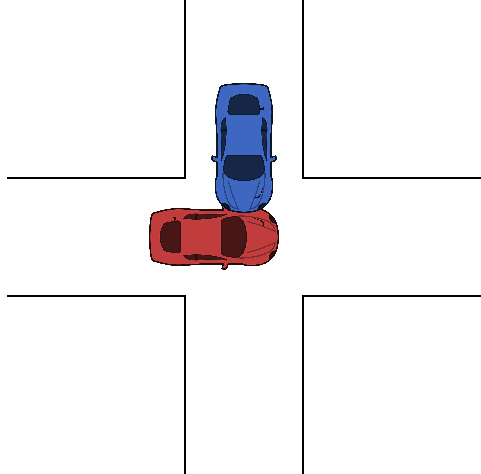
\includegraphics[width=0.7\columnwidth]{YourThesis/papers/ensamble/figures/figures-scen2.pdf}
% 		\caption{$t=1$, DQN and ensemble RPF without confidence criterion.}
% 	\end{subfigure}
	
% 	\vspace{5pt}
	
% 	\begin{subfigure}[t]{0.48\columnwidth}
% 		\centering
% 		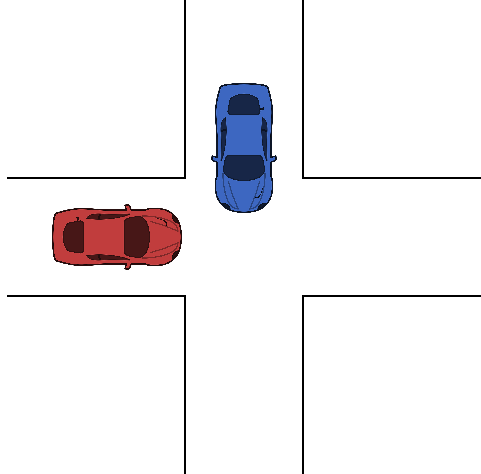
\includegraphics[width=0.7\columnwidth]{YourThesis/papers/ensamble/figures/figures-scen3.pdf}
% 		\caption{$t=1$, ensemble RPF with confidence criterion.}
% 	\end{subfigure}
% 	~ 
% 	\begin{subfigure}[t]{0.48\columnwidth}
% 		\centering
% 		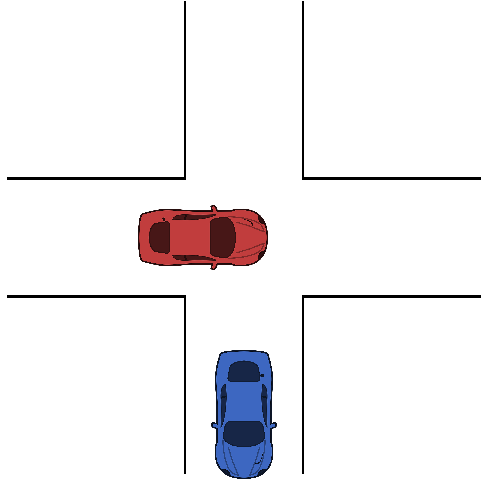
\includegraphics[width=0.7\columnwidth]{YourThesis/papers/ensamble/figures/figures-scen4.pdf}
% 		\caption{$t=1.5$, ensemble RPF with confidence criterion.}
% 	\end{subfigure}
% 	}}
% 	\caption{Example of a situation outside of the training distribution,
% 	where there would be a collision if the confidence criterion is not used. The vehicle at the top is here approaching the crossing at $20$ m/s.}
% 	% \label{fig:collisionOutsideDistribution}

% \end{figure}
\paperBelief show how bad \gls{dqn} is at handing uncertainty in the input space. The results from the experiments show that the algorithms trained with an estimate from the probability distribution outperformed the algorithm trained with the probability distribution as inputs. 

\begin{table}
	\caption{Result summary for 4 cars scenario}
	\label{tab:results_summary}
	\begin{tabularx}{\columnwidth}{@{}l*{10}{c}c@{}}
	\toprule
	Experiments     & Goal reached & Safe stop & Collision & Deadlock & Success time \\ 
			 & $\%$ & $\%$ & $\%$ & $\%$ & s & \\ 
	\midrule
	Oracle DQN    & $84.50$ & $14.45$ & $1.05$ & $0.00$ & $15.49$\\ % $1\unit{\day}7\unit{\hour}$ \\ 
	% Noisy DQN & $84.25$ & $14.10$ & $1.65$ & $0.00$ & $15.48$ \\ 
	\textbf{QMDP-IE}   & $\textbf{80.00}$ & $\textbf{18.15}$ & $\textbf{1.35}$ & $\textbf{0.50}$ & $\textbf{17.14}$ \\ 
	% QMDP-IE   & $80.30$ & $16.20$ & $3.30$ & $0.20$ & $16.54$ & N/A \\ 
	QMDP      & $71.95$ & $15.05$ & $5.70$ & $7.30$ & $20.56$ \\ 
	% \arrayrulecolor{red}\hline
	% \arrayrulecolor{black}
	\textbf{QID}       & $\textbf{85.60}$ & $\textbf{10.40}$ & $\textbf{3.70}$ & $\textbf{0.30}$ & $\textbf{16.64}$ \\ %$\textbf{5\unit{\day}5\unit{\hour}}$ \\ 
	QPF       & $63.50$ & $21.80$ & $12.15$ & $2.55$ & $16.61$ \\ % $5\unit{\day}4\unit{\hour}$\\ 
	
	\bottomrule
	\end{tabularx}
\end{table}

Starting with QMDP-IE, we first demonstrate how the $\zeta_\text{threshold}$ is chosen and then compare its results with QMDP. Both algorithms use the same network weights as the Oracle DQN, but QMPD-IE is less computational than QMDP since the threshold $\zeta_\text{threshold}$ transforms the set of particles into a point estimate of the intention state, as described in \ref{sec:belief_rl_algo}. Therefore, the choice of $\zeta_\text{threshold}$ is an important hyperparameter that directly correlates with the aggressiveness of the agent.

As opposed to QMDP-IE and QMDP, QID and QPF algorithms do not require access to the true intent during training time. While QPF trains a network using all particles, QID only uses the intention distribution from the particles, which reduces the size of the network while keeping information about the uncertainty of the intention state. 
Looking at \ref{tab:results_summary}, QPF has the highest collision rate at \SI{12.15}{\percent} and the second lowest success time out of all considered algorithms, making it the most aggressive policy out of all four algorithms. 
QID collided more than QMDP-IE but still less than QMDP. This shows that training on ground truth is preferred, but QID is a good algorithm to use when ground truth data is not available. 
One downside is that QID and QPF took much longer time to train than the Oracle DQN, with up to 5 days of training. Since QID and QPF have comparable training times, this hints that the particle filter used by both algorithms is the main explanation for the computational time and that the large state space of QPF is of minor importance.

\subsection{Overtake agent}
\begin{table}
\caption{Results with an overtake agent}
\label{tab:results_overtake}
\begin{tabularx}{\columnwidth}{@{}l*{10}{c}c@{}}
\toprule
Experiments & Goal reached & Safe stop & Collision & Deadlock & Success time \\ 
     & $\%$ & $\%$ & $\%$ & $\%$ & s \\ 
\midrule
Oracle DQN & $89.80$ & $0.15$ & $10.05$ & $0.00$ & $16.01$ \\ 
\textbf{QMDP-IE} & $\textbf{94.55}$ & $\textbf{0.20}$ & $\textbf{4.60}$ & $\textbf{0.65}$ & $\textbf{16.62}$ \\ 
QMDP & $79.70$ & $10.20$ & $5.95$ & $4.15$ & $19.84$ \\ 
\textbf{QID} & $\textbf{96.89}$ & $\textbf{0.11}$ & $\textbf{2.53}$ & $\textbf{0.47}$ & $\textbf{16.38}$ \\ 
QPF & $96.15$ & $0.10$ & $3.70$ & $0.05$ & $17.62$ \\ 
\bottomrule
\end{tabularx}
\end{table}

In the overtake scenario, both QID and QPF have relatively low collision rates at \SI{2.53}{\percent} and \SI{3.7}{\percent} respectively, which is lower when compared to the trained scenarios in \ref{tab:results_summary}. 
While the collision rate for QMDP-IE and QMDP is \SI{4.6}{\percent} and \SI{5.95}{\percent} respectively, which is higher than what they got on the trained scenario but it is also higher than QID and QPF. This indicates that QID and QPF are better at handling some scenarios outside the training set than QMDP-IE and QMDP.
QMDP also has the highest safe stop and deadlock rate at \SI{10.2}{\percent} and \SI{4.15}{\percent}, making it the most passive policy. 